\documentclass[journal=jacsat,manuscript=article]{achemso}

% Image-related packages
\usepackage{graphicx}
\usepackage{subcaption}
\usepackage[export]{adjustbox}
\usepackage{wrapfig}

\newcommand*\mycommand[1]{\texttt{\emph{#1}}}

\author{Nayanika Das}
\affiliation[UVicUCC]{Computational Biochemistry and Biophysics Lab, Research Group on Bioinformatics and Bioimaging (BI$^2$), Department of Biosciences, Universitat de Vic - Universitat Central de Catalunya, 08500 Vic, Spain}
\author{Vijay Baladhye}
\affiliation[SPPU]{Savitribai Phule Punr University, Pune, India}
\author{Jordi Villà-Freixa}
\email{jordi.villa@uvic.cat}
\affiliation[UVicUCC]{Computational Biochemistry and Biophysics Lab, Research Group on Bioinformatics and Bioimaging (BI$^2$), Department of Biosciences, Universitat de Vic - Universitat Central de Catalunya, 08500 Vic, Spain}
\alsoaffiliation{IRIS-CC}

\title[Computational analysis of GPX6 activation free energy]
  {Computational analysis of the evolution of glutathione peroxidase 6 (GPX6) activation free energy}

\abbreviations{IR,NMR,UV}
\keywords{Ancestral enzyme reconstruction, enzyme design, empirical valence bond, free energy calculations}

\begin{document}

\begin{abstract}
Outstanding success in computational protein design has been achieved in recent years by combining machine learning approaches with physicochemical properties analysis of the explored variants. Despite these efforts, however, less success has been obtained in designing good computational protocols for optimization of enzyme activity. Here we propose the use of the Empirical Valence Bond method to evaluate free energies of activation of enzyme variants to obtain reasonable mutational pathways leading to a functionally optimized protein. In particular, we propose a method that explores a lower free energy difference pathway for the directed evolution of enzymes based on EVB activation free energies. To test the idea, we study the hypothetical connectivity of the selenocysteine-containing human glutathione peroxidase 6 protein (GPX6) into its ortholog cysteine-containing mouse GPX6. We show how it is possible to find a mutational pathway connecting the two protein sequences and structures that provide the empirical barriers for the first step of the GPX6-catalyzed reaction. Moreover, this protocol offers the potential for addressing complex issues such as epistasis in enzyme engineering, further enhancing its utility in enzyme optimization.
\end{abstract}

\section{Introduction}
Selenium (Se), in the form of selenocysteine (Sec, U—the 21st amino acid) occurs in 25 proteins in the human proteome. Insertion of Sec into a protein is much more complicated than the other 20 amino acids because a UGA stop codon must be recoded as a sense codon for Sec \cite{hondal_differing_2011}. The complexity of this process signifies that Sec must fulfill a chemical function that exerts biological pressure on the genome to maintain the Sec-insertion machinery \cite{hondal_differing_2011,cardey_selenocysteine_2007}. The view of Sec as a sophisticated innovation implies that for each occurrence of Sec in an enzyme there is a unique and specific reason for the use of Se to enhance the enzymatic reaction relative to that of S \cite{hondal_differing_2011}. This view also implies that since Se “speeds reactions” Sec should have widely substituted for Cys in enzymes, which clearly has not occurred. Specific reasons for the usage of Sec might include the enhanced nucleophilic character of Se relative to S, or another might be the much lower pKa of a selenol relative to that of a thiol \cite{hondal_differing_2011}.

Selenium (Se), in the form of selenocysteine (Sec, U—the 21st amino acid) occurs in 25 proteins in the human proteome. Under physiological conditions, inorganic or organic Se is mostly metabolized into selenocysteine (Sec), an amino acid that is then inserted into the primary structure of peptide chains to form selenoproteins \cite{}. Insertion of Sec into a protein is much more complicated than the other 20 amino acids because a UGA stop codon must be recoded as a sense codon for Sec \cite{hondal_differing_2011}. The micronutrient Se is either metabolized through the trans-selenation pathway or via reduction by thioredoxin reductases (TXNRDs) in the presence of glutathione (GSH), depending on the dietary chemical form ingested\cite{}.  The complexity of this process signifies that Sec must fulfill a chemical function that exerts biological pressure on the genome to maintain the Sec-insertion machinery \cite{hondal_differing_2011,cardey_selenocysteine_2007}. The view of Sec as a sophisticated innovation implies that for each occurrence of Sec in an enzyme there is a unique and specific reason for the use of Se to enhance the enzymatic reaction relative to that of S \cite{hondal_differing_2011}. Specific reasons for the usage of Sec might include the enhanced nucleophilic character of Se relative to S, or another might be the much lower pKa of a selenol relative to that of a thiol\cite{hondal_differing_2011}. Besides the fundamental role organoselenides have in organic catalysis, particularly in oxidations of substrates by $H_{2} O_{2}$, selenium-mediated redox reactions are key steps in biological processes related to oxidative stress control and cell signaling \cite{14}. Glutathione peroxidase from class 1 (GPX1, EC 1.11.1.9) is a selenoprotein which protects cells from oxidative damage by catalyzing the reduction of $H_{2} O_{2}$.

Although the catalytic triad of glutathione peroxidase (GPX) has been well recognized, there has been little evidence for the relevance of the interactions among the triad amino acid, i.e. selenocysteine (U), glutamine (Q), and tryptophan (W). Hence, the mechanism of has been studied in various aspects. A catalytic mechanism proposed for GPX3 by Prabhakar et al. based on DFT calculations has the resting state of Sec as selenol, In the first part of this reaction, hydrogen peroxide coordinates to the active site of the enzyme and the proton tranfer is happening to the oxygen atom of Gln residue \cite{prabhakar_elucidation_2005,prabhakar_is_2006}. While another study demonstrated that the ionized selenolate state of Sec in GPX1 is the favorable form for the reduction of hydroperoxide substrates where they modeled the first reaction step of the redox cycle of based on the proposed GPX1-\({\ Sec^-}\)- Arg177 mechanism [8]. Flohe et al. [6]\cite{orian_selenocysteine_2015} explored the mechanism in two different ways wherein the selenocysteine proton moves via water to the indol nitrogen of the Trp residue and then the hydrogen peroxide and with the result of formation of  the products are instantly, without any measurable activation energy. And on the other hand they also explored another path where the hydrogen peroxide was added in the first step of the redox step of the conversion of SeH (selenol) to selenolate ion \({\ Sec^-}\)\cite{flohe_glutathione_2022,orian_selenocysteine_2015}. The most feasible mechanism that we followed here is the SeH-Gln83 by using the implementation of the DFT calculated and experimental values from the reference reaction \cite{prabhakar_is_2006}. 

\subsection{Mechanism of GPX}

A catalytic mechanism proposed for GPX3 by Morokuma et al. involves the formation of a selenolate anion, followed by bond cleavage in hydrogen peroxide leading to the formation of selenenic acid, with a computed barrier of 18.0 kcal/mol \cite{Prabhakar2006}. Flohe et al. propose an alternate mechanism involving charge separation steps \cite{Orian2015}.

\begin{figure}[h]
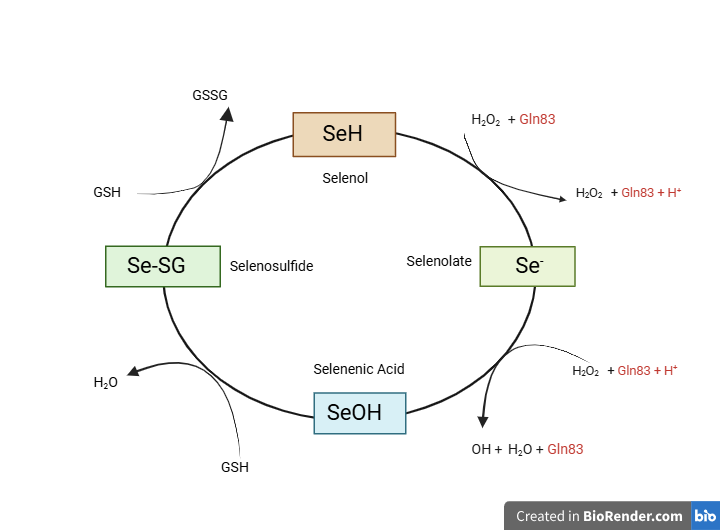
\includegraphics[width=0.7\textwidth]{figures/Catalytic_cycle.png}
\caption{Catalytic Cycle of GPX as given by Morokuma et al. where the resting state of selenium is Selenol}
\label{fig:figure1}
\end{figure}

\subsection{Directed Evolution and Epistasis in Enzyme Design}

Directed evolution mimics natural selection to optimize enzyme traits. Computational design adapts these principles to predict mutation pathways, potentially enhancing enzyme catalytic performance. By exploring mutational pathways with EVB, we investigate the activation energy variations in GPX6 homologs to assess catalytic activity changes due to selenocysteine/cysteine substitution \cite{Starr2016, Storz2018}.

\section{Selection of Variants}

To guide the selection of mutations for directed evolution, a multiple sequence alignment was performed between the human and mouse wild-type protein. This MSA revealed 47 positions that differed between the human and mouse sequences, suggesting potential sites for mutagenesis. In order to prioritize residues for mutagenesis, the distances from the alpha carbon of Cys/Sec49 (active site residue) and rest of the 46 positions were calculated. Residues were then grouped into distance criteria of <10 Å, 10-15 Å, 15-20 Å, 20-25 Å, 25-30 Å, and 30-35 Å. This distance-based approach allowed us to select residues within different proximity ranges to Cys/Sec49. Grouping residues into distance bins provides a systematic and stochastic way to explore the impact of mutations at varying distances from the target residue (Cys/Sec49). We have mutated all these residues one by one slowly changing the human into mouse and the mouse into human structure, in order to understand the changes in the activation barrier in going from proximal to distal mutations in both the structures.

\subsection{Empirical Valence Bond Model based on QM/MM Calculations}

The EVB approach constructs potential energy surfaces for elementary chemical reaction steps \cite{Oanca2024}. Using a two-state model, the EVB Hamiltonian provides insights into thermodynamic activation parameters based on classical force fields and coupling terms derived from DFT or QM/MM calibrations \cite{Oanca2023}.

\section{Computational Model Preparation}

The initial structure used to make the EVB model for mouse cysteine wild type was (PDB ID - 7FC2) and for human selenocysteine wild type it was generated with Alphafold. The parametrization includes in preparing a simulation that has missing force field parameters along with standard parameters and library files. In this case, it is Selenium (U). After equilibration, continuing with the FEP simulations which constitute the core part of the EVB methodology. For creating the selenium parameters (selenol, selenolate ion and selenenic acid), FFLD in Maestro was used. We used the charges provided by Maestro; the hydrogen and solvent were added using the Q program \cite{Marelius1999}. The TIP3P water parameters were used in combination with the other protein parameters not present in the standard OPLS library in Q.

\subsection{Free Energy Calculation Using Q}

Free energy perturbation (FEP) calculations with Q involve running a set of consecutive input files which have the mapping parameter $\lambda$ ranging in a way (usually [1, 0] to [0, 1] between two states). Qfep is a program which reads the energy files generated by Qdyn and calculates the total change in free energy for the complete perturbation from state A ($\varepsilon_1$) to state B ($\varepsilon_2$). Zwanzig’s formula as shown below calculates the difference in free energy between the two states:

\begin{equation}
    \Delta G = \sum \Delta g = \sum -R \cdot T \cdot \ln \left\langle e^{-\left(\frac{\Delta V_{\text{eff}}}{R \cdot T}\right)} \right\rangle_{A}
\end{equation}

Here, \(\Delta V_{\text{eff}}\) is defined as the difference in \( V_{\text{eff}} \) between two adjacent perturbation steps. 

Qfep also calculates free energy functions, or potentials of mean force, using the perturbation formula. The reaction coordinate \(X\) is defined as the energy gap between the states \(X = \Delta V = \varepsilon_1 - \varepsilon_2\) and is divided into intervals \(X_m\) (bins). The first term in the equation represents the free energy difference between the initial state \(\varepsilon_1\) and the mapping potential \(V_i\):

\begin{equation}
    \Delta G(X_m) = \Delta G (\lambda_i) - R \cdot T \cdot \ln \left\langle e^{-\left(\frac{E_g(X_m) - V_i(X_m)}{R \cdot T}\right)} \right\rangle_{i}
\end{equation}

The second term represents the free energy difference between the mapping potential \(V_i\) and the ground state potential \(E_g\). The average in this term is taken over those configurations where \(X\) belongs to \(X_m\).

\begin{equation}
    \Delta G(\lambda_i) = - R \cdot T \cdot \ln \left( \sum_{n=0}^{i-1} \left\langle e^{-\left(\frac{V_{n+1} - V_n}{R \cdot T}\right)} \right\rangle_{n} \right)
\end{equation}

\(E_g\) is the solution to the secular determinant. The system is then represented by an \(n \times n\) EVB Hamiltonian.

\[ 
  \left[\begin{array}{cc}
    H_{11} & H_{12} \\
    H_{21} & H_{22} \\
  \end{array}\right]
\]

Here, \(H_{11}\) and \(H_{22}\) are the energies of the two valence states which are calculated using classical force fields. 
For a two-state representation, the solution becomes:

\begin{equation}
    E_g = \frac{1}{2} \cdot \left( \epsilon_1 + \epsilon_2 \right) - \frac{1}{2} \sqrt{ \left( \epsilon_1 - \epsilon_2 \right)^2 + 4 \cdot H_{12}^2 }
\end{equation}

where \(H_{ij}\) or \(H_{12}\) is the off-diagonal matrix element representing the quantum mechanical coupling of the states. \(H_{ij} \neq 0\) results in the mixing of states \(i\) and \(j\). In Qfep, the off-diagonal element \(H_{ij}\) is a function of the form:

\begin{equation}
    H_{ij} = A_{ij} \cdot e^{-(\mu (r_{ij} - r_0) + \eta (r_{ij} - r_0)^2)}
\end{equation}

The EVB method allows calibration of simulated reference reactions to experimental data obtained from gas-phase or solution experiments. The two EVB parameters \(H_{ij}\) (mostly \(A_{ij}\)) and \(\Delta \alpha\) are adjusted in a way until the calculated profile and the experimental data coincide. The \(\Delta \alpha\) parameter determines the \(\Delta G^\circ\) level, and \(H_{ij}\) regulates the degree of mixing of the states at the transition state, i.e., the \(\Delta G^\ddagger\) level.

\subsection{EVB simulations}

Spherical boundary conditions \cite{King1989} were applied to the system using Q program \cite{Marelius1999} with a 50 \text{\AA} diameter water sphere surrounding the protein.

After equilibration of the system, EVB free energy perturbation (FEP) calculations were done for the step 1 (until formation of selenolate ion). The FEP protocol involves a gradual change of the (mapping) potential energy by the coupling parameter. For each of the FEP calculations, 51 discrete windows were considered, each window of 10 ps at 2 fs time step, that gave a total of 1.02 ns of sampling of each free energy profile. These calculations were replicated 100 times starting from the minimized structure for each of the systems, wild type and mutants. The EVB gas phase shift $\alpha$ and the off-diagonal \(H_{ij}\) were determined iteratively for all systems keeping human selenocysteine as our reference, the barrier was determined according to the QM/MM calculations carried out by Morokuma \cite{Prabhakar2006} for the first step of reaction which was 16.4 kcal/mol.
\begin{figure}
\begin{center}
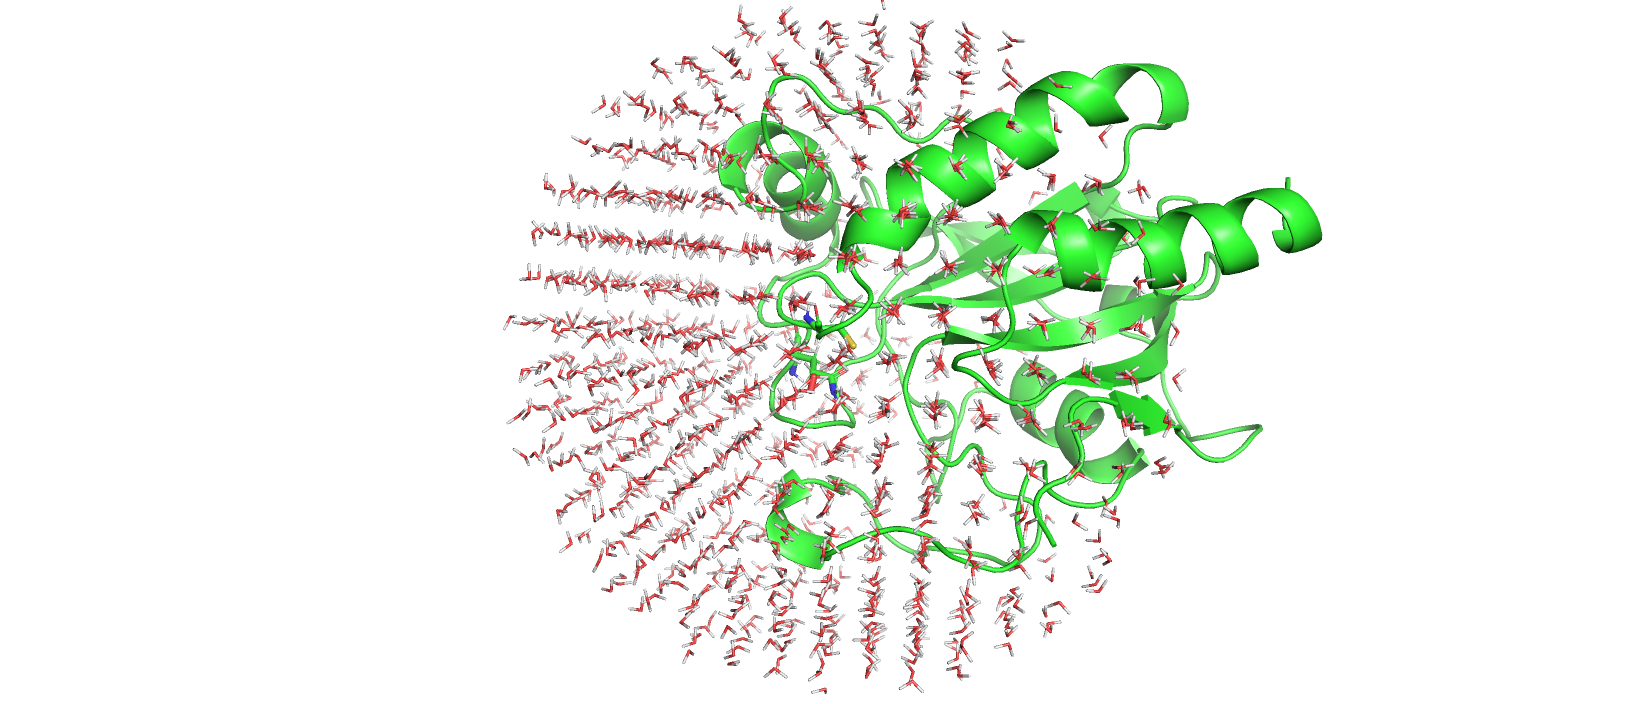
\includegraphics[width=0.7\linewidth, height=5cm]{figures/solvent_sphere.png} 
\end{center}
\caption{Sphere of water molecules around the protein}
\label{fig:figure6}
\end{figure}

\medskip

\bibliographystyle{unsrt}
\bibliography{/home/hp/nayanika/github/GPX6/manuscript/references}


\end{document}
